\begin{figure}[h]
	\centering

	\begin{tikzpicture}
		\begin{axis}[
			view={0}{90},
			title=Operator ${==}$,
			width=0.45\textwidth,
			colormap/hot,
			xticklabels={number,string,undefined,object,null,boolean,function,array},
			xtick={0,...,7},
			yticklabels={number,string,undefined,object,null,boolean,function,array},
			ytick={7,...,0},
			x tick label style={rotate=90,anchor=east}]
		]
		\addplot3[surf, shader=interp, left] file {figures/experiments/operators/equality-operators/operator_==.dat};
		\end{axis}
	\end{tikzpicture}
	%
	\begin{tikzpicture}
		\begin{axis}[
			view={0}{90},
			width=0.45\textwidth,
			title=Operator ${!=}$,
			colormap/hot,
			xticklabels={number,string,undefined,object,null,boolean,function,array},
			xtick={0,...,7},
			yticklabels={number,string,undefined,object,null,boolean,function,array},
			ytick={7,...,0},
			x tick label style={rotate=90,anchor=east}]
		\addplot3[surf, shader=interp, left] file {figures/experiments/operators/equality-operators/operator_!=.dat};
		\end{axis}
	\end{tikzpicture}

	\centering
	\begin{tikzpicture}
		\begin{axis}[
			view={0}{90},
			width=0.45\textwidth,
			title=Operator ${===}$,
			colormap/hot,
			xticklabels={number,string,undefined,object,null,boolean,function,array},
			xtick={0,...,7},
			yticklabels={number,string,undefined,object,null,boolean,function,array},
			ytick={7,...,0},
			x tick label style={rotate=90,anchor=east}]
		\addplot3[surf, shader=interp, left] file {figures/experiments/operators/equality-operators/operator_===.dat};
		\end{axis}
	\end{tikzpicture}
	%
	\begin{tikzpicture}
		\begin{axis}[
			view={0}{90},
			width=0.45\textwidth,
			title=Operator ${!==}$,
			colormap/hot,
			xticklabels={number,string,undefined,object,null,boolean,function,array},
			xtick={0,...,7},
			yticklabels={number,string,undefined,object,null,boolean,function,array},
			ytick={7,...,0},
			x tick label style={rotate=90,anchor=east}]
		\addplot3[surf, shader=interp, left] file {figures/experiments/operators/equality-operators/operator_!==.dat};
		\end{axis}
	\end{tikzpicture}

	\centering
	\hspace{0.1\textwidth}
	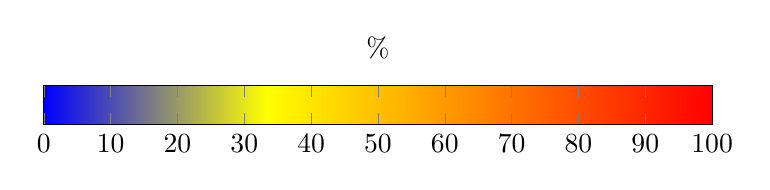
\begin{tikzpicture}
		\begin{axis}[
			hide axis,
			scale only axis,
			height=0pt,
			width=0pt,
			colormap/hot,
			colorbar horizontal,
			point meta min=0,
			point meta max=100,
			colorbar style={
				title=\%,
				width=0.7\textwidth,
				xtick={0, 10, 20, 30, 40, ..., 100}
			}]
			\addplot [draw=none] coordinates {(0,0)};
		\end{axis}
	\end{tikzpicture}
	\caption[Relational operators]{
		\textbf{Type distribution for equality operators} - Operator ${==}$ is mainly used for number comparison. String comparison is performed by using ${===}$ and ${!==}$ operators. Comparison against \textit{null} is performed by using both ${!=}$ and ${!==}$ operators
	}
\end{figure}